\documentclass{beamer}\usepackage[]{graphicx}\usepackage[]{color}
%% maxwidth is the original width if it is less than linewidth
%% otherwise use linewidth (to make sure the graphics do not exceed the margin)
\makeatletter
\def\maxwidth{ %
  \ifdim\Gin@nat@width>\linewidth
    \linewidth
  \else
    \Gin@nat@width
  \fi
}
\makeatother

\definecolor{fgcolor}{rgb}{0.345, 0.345, 0.345}
\newcommand{\hlnum}[1]{\textcolor[rgb]{0.686,0.059,0.569}{#1}}%
\newcommand{\hlstr}[1]{\textcolor[rgb]{0.192,0.494,0.8}{#1}}%
\newcommand{\hlcom}[1]{\textcolor[rgb]{0.678,0.584,0.686}{\textit{#1}}}%
\newcommand{\hlopt}[1]{\textcolor[rgb]{0,0,0}{#1}}%
\newcommand{\hlstd}[1]{\textcolor[rgb]{0.345,0.345,0.345}{#1}}%
\newcommand{\hlkwa}[1]{\textcolor[rgb]{0.161,0.373,0.58}{\textbf{#1}}}%
\newcommand{\hlkwb}[1]{\textcolor[rgb]{0.69,0.353,0.396}{#1}}%
\newcommand{\hlkwc}[1]{\textcolor[rgb]{0.333,0.667,0.333}{#1}}%
\newcommand{\hlkwd}[1]{\textcolor[rgb]{0.737,0.353,0.396}{\textbf{#1}}}%
\let\hlipl\hlkwb

\usepackage{framed}
\makeatletter
\newenvironment{kframe}{%
 \def\at@end@of@kframe{}%
 \ifinner\ifhmode%
  \def\at@end@of@kframe{\end{minipage}}%
  \begin{minipage}{\columnwidth}%
 \fi\fi%
 \def\FrameCommand##1{\hskip\@totalleftmargin \hskip-\fboxsep
 \colorbox{shadecolor}{##1}\hskip-\fboxsep
     % There is no \\@totalrightmargin, so:
     \hskip-\linewidth \hskip-\@totalleftmargin \hskip\columnwidth}%
 \MakeFramed {\advance\hsize-\width
   \@totalleftmargin\z@ \linewidth\hsize
   \@setminipage}}%
 {\par\unskip\endMakeFramed%
 \at@end@of@kframe}
\makeatother

\definecolor{shadecolor}{rgb}{.97, .97, .97}
\definecolor{messagecolor}{rgb}{0, 0, 0}
\definecolor{warningcolor}{rgb}{1, 0, 1}
\definecolor{errorcolor}{rgb}{1, 0, 0}
\newenvironment{knitrout}{}{} % an empty environment to be redefined in TeX

\usepackage{alltt}
\IfFileExists{upquote.sty}{\usepackage{upquote}}{}
\begin{document}

\title{Data wrangling and Wordcloud}
\author{Akhilesh Atluri}

\begin{frame}
  \titlepage
\end{frame}

\begin{frame}
  \frametitle{Outline}
    \tableofcontents
\end{frame}

\section{Install and Load Libraries}
\begin{frame}[fragile]
  \frametitle{Install and Load Libraries}
    \begin{itemize}
      \item<1->
\begin{knitrout}
\definecolor{shadecolor}{rgb}{0.969, 0.969, 0.969}\color{fgcolor}\begin{kframe}
\begin{alltt}
\hlkwd{library}\hlstd{(dplyr)}
\end{alltt}
\end{kframe}
\end{knitrout}
      \item<2->
\begin{knitrout}
\definecolor{shadecolor}{rgb}{0.969, 0.969, 0.969}\color{fgcolor}\begin{kframe}
\begin{alltt}
\hlkwd{library}\hlstd{(tidytext)}
\end{alltt}
\end{kframe}
\end{knitrout}
    \item<3->
\begin{knitrout}
\definecolor{shadecolor}{rgb}{0.969, 0.969, 0.969}\color{fgcolor}\begin{kframe}
\begin{alltt}
\hlkwd{library}\hlstd{(gutenbergr)}
\end{alltt}
\end{kframe}
\end{knitrout}
    \item<4->
\begin{knitrout}
\definecolor{shadecolor}{rgb}{0.969, 0.969, 0.969}\color{fgcolor}\begin{kframe}
\begin{alltt}
\hlkwd{library}\hlstd{(ggplot2)}
\end{alltt}
\end{kframe}
\end{knitrout}
    \item<5->
\begin{knitrout}
\definecolor{shadecolor}{rgb}{0.969, 0.969, 0.969}\color{fgcolor}\begin{kframe}
\begin{alltt}
\hlkwd{library}\hlstd{(stringr)}
\end{alltt}
\end{kframe}
\end{knitrout}
    \item<6->
\begin{knitrout}
\definecolor{shadecolor}{rgb}{0.969, 0.969, 0.969}\color{fgcolor}\begin{kframe}
\begin{alltt}
 \hlkwd{library}\hlstd{(wordcloud)}
\end{alltt}
\end{kframe}
\end{knitrout}
    \end{itemize}
\end{frame}

\section{Getting the data from Gutenbergr}

\begin{frame}[fragile] 

  \frametitle{Getting the data from Gutenbergr}
\begin{knitrout}
\definecolor{shadecolor}{rgb}{0.969, 0.969, 0.969}\color{fgcolor}\begin{kframe}
\begin{alltt}
\hlkwd{gutenberg_works}\hlstd{(}\hlkwd{str_detect}\hlstd{(title,}\hlstr{'The Adventure'}\hlstd{))}
\end{alltt}
\begin{verbatim}
## # A tibble: 171 x 8
##    gutenberg_id
##           <int>
##  1           74
##  2          500
##  3          909
##  4         1194
##  5         1218
##  6         1372
##  7         1644
##  8         1661
##  9         1825
## 10         2343
## # ... with 161 more rows, and 7 more variables: title <chr>, author <chr>,
## #   gutenberg_author_id <int>, language <chr>, gutenberg_bookshelf <chr>,
## #   rights <chr>, has_text <lgl>
\end{verbatim}
\begin{alltt}
\hlstd{sherlock}\hlkwb{<-}\hlkwd{gutenberg_download}\hlstd{(}\hlnum{1661}\hlstd{)}
\end{alltt}


{\ttfamily\noindent\itshape\color{messagecolor}{\#\# Determining mirror for Project Gutenberg from http://www.gutenberg.org/robot/harvest}}

{\ttfamily\noindent\itshape\color{messagecolor}{\#\# Using mirror http://aleph.gutenberg.org}}\end{kframe}
\end{knitrout}
\end{frame}


\section{Getting the words}

\begin{frame}[fragile] 

  \frametitle{Getting the words}
\begin{knitrout}
\definecolor{shadecolor}{rgb}{0.969, 0.969, 0.969}\color{fgcolor}\begin{kframe}
\begin{alltt}
\hlstd{sherlock_words}\hlkwb{<-}\hlstd{sherlock}\hlopt
  \hlkwd{unnest_tokens}\hlstd{(word,text)}
\hlstd{sherlock_words}
\end{alltt}
\begin{verbatim}
## # A tibble: 105,426 x 2
##    gutenberg_id       word
##           <int>      <chr>
##  1         1661        the
##  2         1661 adventures
##  3         1661         of
##  4         1661   sherlock
##  5         1661     holmes
##  6         1661         by
##  7         1661        sir
##  8         1661     arthur
##  9         1661      conan
## 10         1661      doyle
## # ... with 105,416 more rows
\end{verbatim}
\end{kframe}
\end{knitrout}
\end{frame}

\section{Getting rid of unwanted words}

\begin{frame}[fragile] 

  \frametitle{Getting rid of unwanted words}
\begin{knitrout}
\definecolor{shadecolor}{rgb}{0.969, 0.969, 0.969}\color{fgcolor}\begin{kframe}
\begin{alltt}
\hlstd{sherlock_words}\hlkwb{<-}\hlstd{sherlock_words}\hlopt
  \hlkwd{filter}\hlstd{(}\hlopt{!}\hlstd{(word} \hlopt \hlstd{stop_words}\hlopt{$}\hlstd{word))}
\end{alltt}
\end{kframe}
\end{knitrout}
\end{frame}

\section{grouping each word and getiing the count of each word}

\begin{frame}[fragile] 

  \frametitle{grouping each word and getiing the count of each word}
\begin{knitrout}
\definecolor{shadecolor}{rgb}{0.969, 0.969, 0.969}\color{fgcolor}\begin{kframe}
\begin{alltt}
\hlstd{sherlock_freq}\hlkwb{<-}\hlstd{sherlock_words}\hlopt
  \hlkwd{group_by}\hlstd{(word)}\hlopt
  \hlkwd{summarize}\hlstd{(}\hlkwc{count}\hlstd{=}\hlkwd{n}\hlstd{())}
\end{alltt}
\end{kframe}
\end{knitrout}
\end{frame}

\section{displaying the words on wordlcoud}

\begin{frame}[fragile] 

  \frametitle{displaying the words on wordcloud}
\begin{knitrout}
\definecolor{shadecolor}{rgb}{0.969, 0.969, 0.969}\color{fgcolor}\begin{kframe}
\begin{alltt}
\hlkwd{wordcloud}\hlstd{(sherlock_freq}\hlopt{$}\hlstd{word,sherlock_freq}\hlopt{$}\hlstd{count,}\hlkwc{min.freq} \hlstd{=} \hlnum{25}\hlstd{)}
\end{alltt}
\end{kframe}
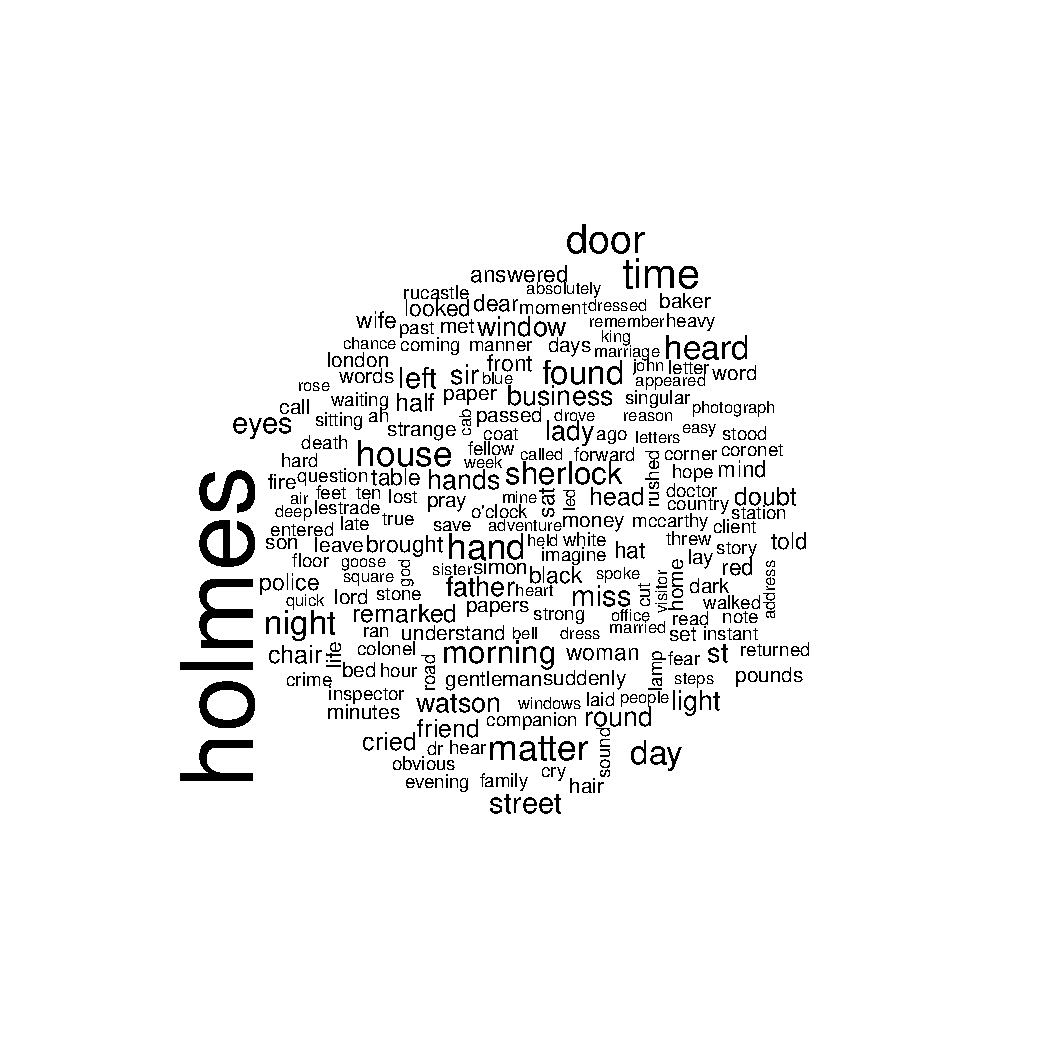
\includegraphics[width=\maxwidth]{figure/unnamed-chunk-11-1} 

\end{knitrout}
\end{frame}
\end{document}
